\documentclass[tikz,border=1mm]{standalone}
\usepackage[T1]{fontenc}
\usepackage{helvet}
\renewcommand{\familydefault}{\sfdefault}
\usetikzlibrary{arrows.meta,calc}

\definecolor{heat}{HTML}{A75231}
\definecolor{payment}{HTML}{315B7C}
\definecolor{ink}{HTML}{303A40}
\definecolor{muted}{HTML}{657078}
\definecolor{rule}{HTML}{D2D8DC}
\definecolor{papergray}{HTML}{F6F7F8}

% Publication layout: 180 mm overall width, including the standalone border.
% All labels are live text. Colour identifies arrows and keys, not body text.
%
% Scientific scope and source notes:
% 1. This is a heat-flow and institutional schematic, not a hydraulic drawing.
%    The requested upper/lower-third connections are graphical energy ports.
%    They do NOT represent diffuser elevations or imply hot-water withdrawal
%    from the bottom. VEKS describes hot-water discharge from the top, with
%    return water entering the bottom. Return circuits and storage HX omitted.
% 2. The inset depicts Varmelast's published system-level message sequence.
%    Its timestamps describe system planning, not a verified PTES-specific
%    notification deadline. Times are local. PTES look-ahead is shown separately.
% 3. HTF demand information and local operation follow the project account.
%    The forecast arrow is an institutional information link, not a claim about
%    a direct IT interface. Public Varmelast forecasts cover VEKS/CTR/HOFOR areas.
% 4. Shading distinguishes physical networks, not ownership. PTES is joint.
% 5. The monthly tariff and pumping expense follow project evidence.
%    Storage-rights compensation is also documented by PlanEnergi.
%
% Public sources:
% https://www.varmelast.dk/lastfordeling/varmeplaner
% https://www.varmelast.dk/lastfordeling/varmebehov
% https://www.varmelast.dk/fjernvarmesystemet/brug-af-varmelagre
% https://www.veks.dk/-/media/veks/files/publications/damvarmelager-folder
%
% Design references: Elsevier artwork sizing and Nature research figure guide.
% These inform legibility, editable vector output and restrained styling;
% this figure is not claimed to meet every journal-specific house rule.

\begin{document}
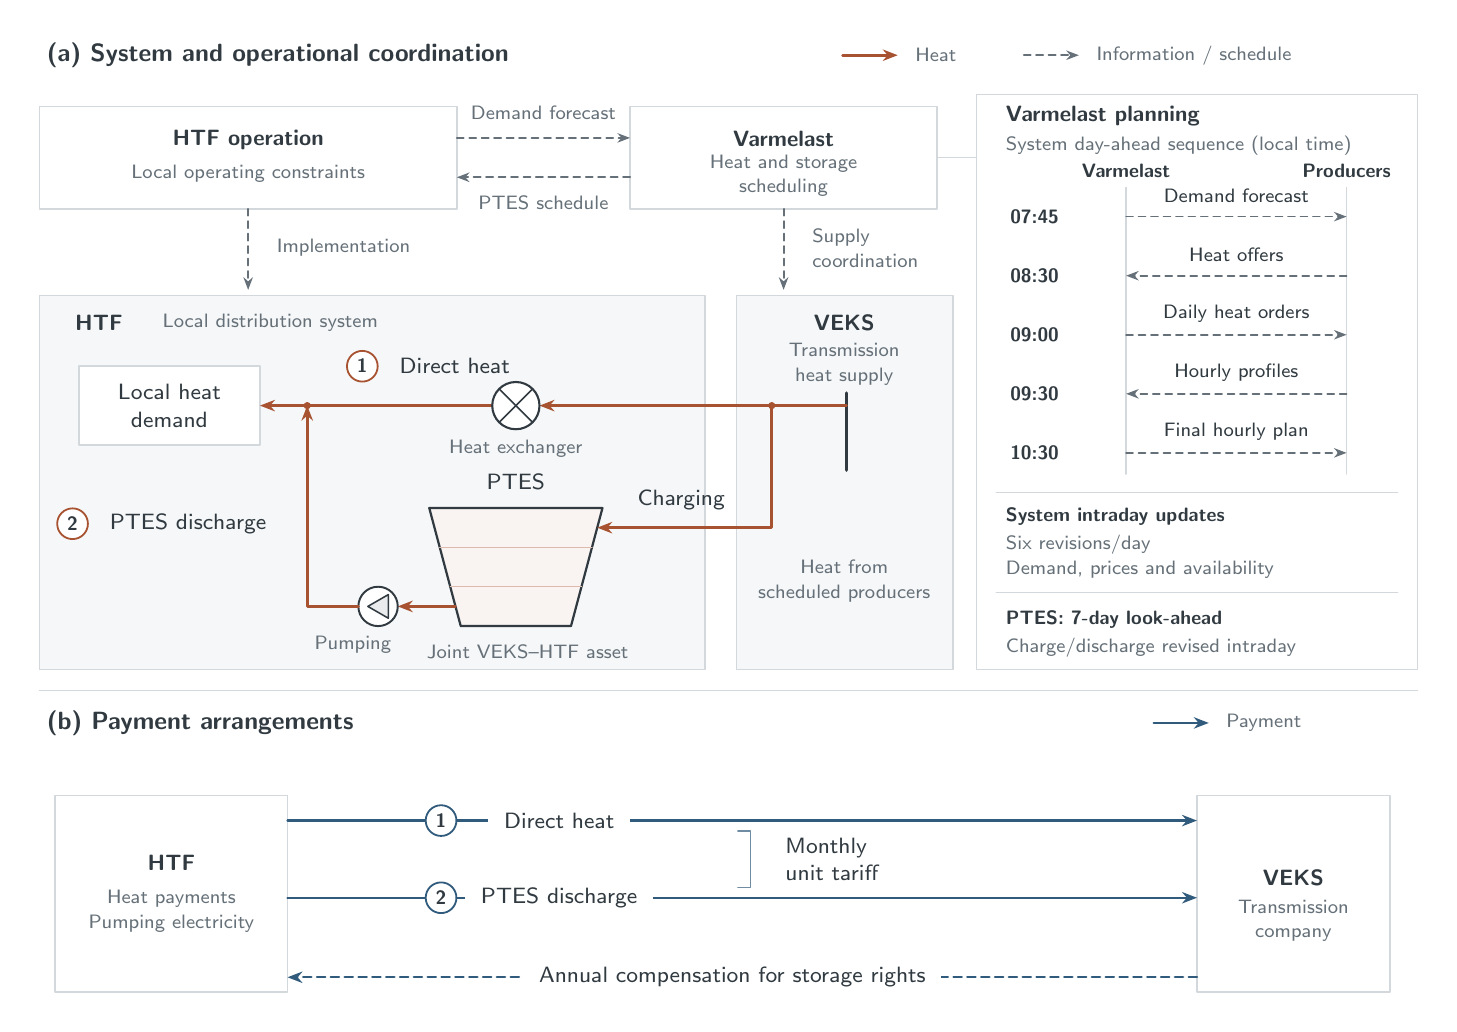
\begin{tikzpicture}[
  x=1cm,y=1cm,
  font=\fontsize{8.25}{10}\selectfont,text=ink,
  line cap=round,line join=round,
  panel/.style={anchor=west,font=\bfseries\fontsize{9}{11}\selectfont},
  actor/.style={font=\bfseries\fontsize{8.5}{10.3}\selectfont},
  small/.style={font=\fontsize{7.3}{8.9}\selectfont,text=muted},
  supplyarea/.style={draw=rule,line width=.5pt,fill=papergray},
  heatflow/.style={draw=heat,line width=1.0pt,
    -{Stealth[length=1.9mm,width=1.45mm]}},
  cashflow/.style={draw=payment,line width=.85pt,
    -{Stealth[length=1.9mm,width=1.45mm]}},
  coordination/.style={draw=muted,line width=.7pt,
    dash pattern=on 2.5pt off 2pt,
    -{Stealth[length=1.6mm,width=1.2mm]}},
  card/.style={draw=rule,line width=.6pt,fill=white,
    minimum height=1.10cm,inner sep=0pt},
  inline/.style={fill=white,inner xsep=2mm,inner ysep=1mm},
  route/.style={circle,draw=heat,line width=.65pt,fill=white,
    text=ink,font=\bfseries\fontsize{7.3}{8}\selectfont,
    minimum size=3.9mm,inner sep=0pt},
  payroute/.style={route,draw=payment},
  time/.style={anchor=east,font=\bfseries\fontsize{7.5}{9}\selectfont},
  event/.style={anchor=west,align=left,text width=3.65cm,
    inner sep=0pt,font=\fontsize{7.3}{8.9}\selectfont},
]
\path[use as bounding box] (0,1.30) rectangle (17.8,13.70);

% ------------------------------------------------------------------
% (a) Local demand, central planning, and physical heat delivery
% ------------------------------------------------------------------
\node[panel] at (.12,13.35) {(a) System and operational coordination};
\draw[heatflow] (10.35,13.35) -- (11.05,13.35);
\node[small,anchor=west] at (11.15,13.35) {Heat};
\draw[coordination] (12.65,13.35) -- (13.35,13.35);
\node[small,anchor=west] at (13.45,13.35) {Information / schedule};

% Local information goes to Varmelast; the storage schedule returns to HTF.
\node[card,minimum width=5.30cm,minimum height=1.30cm]
  (operator) at (2.80,12.05) {};
\node[actor] at (2.80,12.27) {HTF operation};
\node[small] at (2.80,11.85) {Local operating constraints};
\node[card,minimum width=3.90cm,minimum height=1.30cm]
  (scheduler) at (9.60,12.05) {};
\node[actor] at (9.60,12.29) {Varmelast};
\node[small,align=center] at (9.60,11.82) {Heat and storage\\scheduling};

\draw[coordination] (5.45,12.30) -- (7.65,12.30);
\node[small] at (6.55,12.62) {Demand forecast};
\draw[coordination] (7.65,11.80) -- (5.45,11.80);
\node[small] at (6.55,11.47) {PTES schedule};
\draw[coordination] (2.80,11.40) -- (2.80,10.37);
\node[small,anchor=west] at (3.04,10.90) {Implementation};
\draw[coordination] (9.60,11.40) -- (9.60,10.37);
\node[small,anchor=west,align=left] at (9.84,10.90) {Supply\\coordination};

% The inset is a system-level message sequence, not a PTES-specific algorithm.
% Actor columns and labelled exchanges distinguish processes from time-series
% information, following the visual grammar of the reviewed Frigg papers.
\path[draw=rule,line width=.55pt,fill=white]
  (12.05,5.55) rectangle (17.65,12.85);
\draw[rule,line width=.55pt] (11.55,12.05) -- (12.05,12.05);
\node[actor,anchor=west] at (12.30,12.58) {Varmelast planning};
\node[small,anchor=west] at (12.30,12.20) {System day-ahead sequence (local time)};

% Columns identify sender and receiver; their vertical rules are not flows.
\node[font=\bfseries\fontsize{7.3}{8.9}\selectfont]
  at (13.95,11.88) {Varmelast};
\node[font=\bfseries\fontsize{7.3}{8.9}\selectfont]
  at (16.75,11.88) {Producers};
\draw[rule,line width=.45pt] (13.95,8.03) -- (13.95,11.67);
\draw[rule,line width=.45pt] (16.75,8.03) -- (16.75,11.67);

% Day-ahead exchanges as published by Varmelast.
\node[time] at (13.22,11.30) {07:45};
\draw[coordination,line width=.6pt] (13.95,11.30) -- (16.75,11.30);
\node[font=\fontsize{7.3}{8.9}\selectfont] at (15.35,11.57) {Demand forecast};

\node[time] at (13.22,10.55) {08:30};
\draw[coordination,line width=.6pt] (16.75,10.55) -- (13.95,10.55);
\node[font=\fontsize{7.3}{8.9}\selectfont] at (15.35,10.82) {Heat offers};

\node[time] at (13.22,9.80) {09:00};
\draw[coordination,line width=.6pt] (13.95,9.80) -- (16.75,9.80);
\node[font=\fontsize{7.3}{8.9}\selectfont] at (15.35,10.07) {Daily heat orders};

\node[time] at (13.22,9.05) {09:30};
\draw[coordination,line width=.6pt] (16.75,9.05) -- (13.95,9.05);
\node[font=\fontsize{7.3}{8.9}\selectfont] at (15.35,9.32) {Hourly profiles};

\node[time] at (13.22,8.30) {10:30};
\draw[coordination,line width=.6pt] (13.95,8.30) -- (16.75,8.30);
\node[font=\fontsize{7.3}{8.9}\selectfont] at (15.35,8.57) {Final hourly plan};

% System intraday cadence is separated from the PTES planning horizon.
\draw[rule,line width=.4pt] (12.30,7.80) -- (17.40,7.80);
\node[anchor=west,font=\bfseries\fontsize{7.5}{9}\selectfont]
  at (12.30,7.49) {System intraday updates};
\node[small,anchor=west] at (12.30,7.14) {Six revisions/day};
\node[small,anchor=west] at (12.30,6.82) {Demand, prices and availability};
\draw[rule,line width=.4pt] (12.30,6.53) -- (17.40,6.53);
\node[anchor=west,font=\bfseries\fontsize{7.5}{9}\selectfont]
  at (12.30,6.18) {PTES: 7-day look-ahead};
\node[small,anchor=west] at (12.30,5.82) {Charge/discharge revised intraday};

% Physical domains: HTF at left, VEKS transmission supply at right.
\path[supplyarea] (.15,5.55) rectangle (8.60,10.30);
\path[supplyarea] (9.00,5.55) rectangle (11.75,10.30);
\node[actor,anchor=west] at (.48,9.95) {HTF};
\node[small,anchor=west] at (1.59,9.95) {Local distribution system};
\node[actor] at (10.37,9.95) {VEKS};
\node[small,align=center] at (10.37,9.43) {Transmission\\heat supply};
\draw[ink,line width=1.2pt] (10.40,8.08) -- (10.40,9.06);
\node[small,align=center] at (10.37,6.67) {Heat from\\scheduled producers};
\node[card,minimum width=2.30cm,minimum height=1.00cm]
  (demand) at (1.80,8.90) {};
\node[align=center] at (1.80,8.90) {Local heat\\demand};

% Route 1: right-to-left delivery through the ordinary heat exchanger.
\draw[heatflow] (10.40,8.90) -- (6.50,8.90);
\draw[heatflow] (5.90,8.90) -- (2.95,8.90);
\draw[ink,line width=.75pt,fill=white] (6.20,8.90) circle (.30);
\draw[ink,line width=.6pt]
  (5.99,8.69) -- (6.41,9.11)
  (5.99,9.11) -- (6.41,8.69);
\node[small] at (6.20,8.35) {Heat exchanger};
\node[route] at (4.25,9.40) {1};
\node[anchor=west] at (4.60,9.40) {Direct heat};

% Route 2: graphical energy ports centred in the top and bottom thirds.
% Pit: top y=7.60, bottom y=6.10, height H=1.50 cm.
% Charge: y=top-H/6=7.35; discharge: y=bottom+H/6=6.35.
% Wall intersections are calculated from the linear trapezoid slopes.
\node at (6.20,7.93) {PTES};
\path[draw=ink,line width=.8pt,fill=heat!7]
  (5.10,7.60) -- (7.30,7.60) -- (6.90,6.10)
  -- (5.50,6.10) -- cycle;
\draw[heat!40,line width=.45pt]
  (5.233333,7.10) -- (7.166667,7.10)
  (5.366667,6.60) -- (7.033333,6.60);
\fill[heat] (9.45,8.90) circle (1.3pt);
\draw[heatflow] (9.45,8.90) -- (9.45,7.35) -- (7.233333,7.35);
\node at (8.30,7.70) {Charging};
\node[small] at (6.35,5.78) {Joint VEKS--HTF asset};

\draw[heatflow] (5.433333,6.35) -- (4.70,6.35);
\draw[ink,line width=.7pt,fill=white] (4.45,6.35) circle (.25);
\path[draw=ink,line width=.55pt,fill=ink!10]
  (4.58,6.20) -- (4.32,6.35) -- (4.58,6.50) -- cycle;
\draw[heatflow] (4.20,6.35) -- (3.55,6.35) -- (3.55,8.90);
\fill[heat] (3.55,8.90) circle (1.3pt);
\node[route] at (.57,7.40) {2};
\node[anchor=west] at (.92,7.40) {PTES discharge};
\node[small] at (4.13,5.86) {Pumping};

% ------------------------------------------------------------------
% (b) Settlement: same left-right actors as the physical arrangement
% ------------------------------------------------------------------
\draw[rule,line width=.5pt] (.15,5.28) -- (17.65,5.28);
\node[panel] at (.12,4.87) {(b) Payment arrangements};
\draw[cashflow] (14.30,4.87) -- (15.00,4.87);
\node[small,anchor=west] at (15.10,4.87) {Payment};

\node[card,minimum width=2.95cm,minimum height=2.50cm]
  (htfcash) at (1.825,2.70) {};
\node[actor] at (1.825,3.10) {HTF};
\node[small,align=center] at (1.825,2.48)
  {Heat payments\\Pumping electricity};
\node[card,minimum width=2.45cm,minimum height=2.50cm]
  (vekscash) at (16.075,2.70) {};
\node[actor] at (16.075,2.90) {VEKS};
\node[small,align=center] at (16.075,2.36) {Transmission\\company};

\draw[cashflow] (3.30,3.63) -- (14.85,3.63);
\node[payroute] at (5.25,3.63) {1};
\node[inline] at (6.75,3.63) {Direct heat};
\draw[cashflow] (3.30,2.65) -- (14.85,2.65);
\node[payroute] at (5.25,2.65) {2};
\node[inline] at (6.75,2.65) {PTES discharge};
\draw[payment!70,line width=.55pt]
  (9.02,3.50) -- (9.18,3.50) -- (9.18,2.78) -- (9.02,2.78);
\node[anchor=west,align=left] at (9.50,3.14) {Monthly\\unit tariff};
\draw[cashflow,dash pattern=on 3pt off 2pt] (14.85,1.64) -- (3.30,1.64);
\node[inline] at (8.95,1.64) {Annual compensation for storage rights};

\end{tikzpicture}
\end{document}

% Suggested descriptive manuscript caption:
% Physical arrangement, operating coordination and payment arrangements for
% the H\o{}je Taastrup pit thermal energy storage (PTES). (a) HTF receives
% heat directly through the heat exchanger (1) or through PTES discharge (2).
% Charging heat is supplied from the VEKS transmission system. The inset
% distinguishes the published system-level day-ahead exchanges between
% Varmelast and producers, the system intraday revision cadence, and the
% PTES seven-day planning horizon with intraday charging/discharging updates.
% The day-ahead times are not asserted to be PTES notification deadlines.
% (b) Both delivery routes face a common monthly unit tariff; HTF incurs the
% indicated pumping electricity expenditure, and receives separate annual
% compensation from VEKS for storage rights. Heat and information flows are
% schematic. Energy-port heights are illustrative, not diffuser elevations;
% return circuits, storage heat exchangers and other local sources are omitted.
% Shaded regions indicate the physical supply networks, not asset ownership.
%
% Figure-design references reviewed:
% Schledorn et al. (2022), Applied Energy 317, 119074, Figs. 1--2.
% Schledorn et al. (2024), Applied Energy 364, 122960, graphical abstract.
% Dominkovic et al. (2020), Applied Energy 260, 114292, Fig. 2.
% The figure is an independent schematic; no published artwork is reproduced.
%
% Scheduling sources:
% https://www.varmelast.dk/lastfordeling/varmeplaner
% https://www.varmelast.dk/fjernvarmesystemet/brug-af-varmelagre
% https://ens.dk/media/7413/download (PlanEnergi 2025, printed p.24).
% The last source documents seven-day PTES optimisation and intraday plans
% that may supersede the longer plan; it does not disclose a full algorithm.
% Use project evidence for the heat-tariff and local implementation details.
